\section{Durchführung}
\label{sec:Durchführung}
\subsection{Aufbau}

\begin{figure}
    \centering
    \caption{Der Aufbau des Versuchs. Das Bild stammt aus Quelle \cite{anleitung}.}
    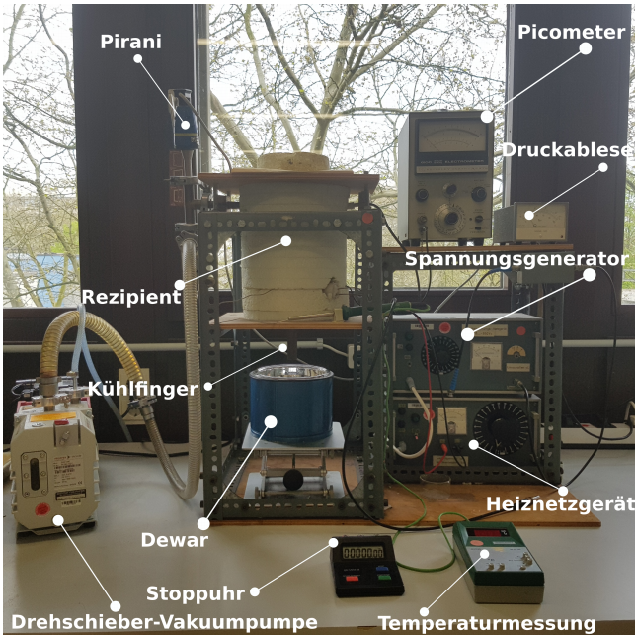
\includegraphics[width=\textwidth]{content/data/Aufbau.png}
    \label{fig:aufbau}
\end{figure}

Der Aufbau des Versuchs ist in \autoref{fig:aufbau} zu finden.
Er besteht aus einen Vakuumgefäß, dem so genannten Rezipienten, indem sich die Probe befindet.
An den Rezipienten ist eine Vakuumpumpe angeschlossen, sodass das Vakuum auf einem konstanten Wert bleibt.
Das Vakuum ist wichtig da die Probe hygroskopisch sind und sich so auf dem Kistall Wasser absetzen würde.
Die Wassermolkühle stören allerdings im Versuch, da sie Dipoleigenschaften besitzen und mit den Dipolen im Kristall wechselwirken.
\\\\
Die Probe im Rezipienten besteht aus Kalium-Bromid (KBr).
Diese ruht auf einer Metallplatte die wiederrum mit einem Kühlfinger, einer Heizspule und einem Thermofühler verbunden ist.
So kann die Temperatur des Probenkristalls reguliert werden.
Um die Probe zu kühlen steht ein Dewar-Gefäß unter dem Kühlfinger, welches mit flüssigem Stickstoff gefüllt werden kann.
Um die Probe hingegen zu erwärmen wird das Dewar-Gefäß entfernt und die Heispule wird mit Strom versorgt.
\\\\
Über der Probe befindet sich eine weitere Metallplatte, welche mit der Platte auf der die Probe liegt einen Plattenkondensator bildet.
An diesen kann eine Spannung angeschlossen werden um die Dipole im Kristall auszurichten.
Außerdem kann der Plattenkondensator an ein Picoampermeter angeschlossen werden um den, durch die Dipolrelaxation, induzierten Strom zu messen.

\subsection{Ablauf}
Zunächst wird der Plattenkondensator mit einer Spannung von $V = \SI{950}{\V}$ versetzt um die Dipole auszurichten.
Dabei wird der Kristall auf eine Temperatur von $T = \SI{320}{\K}$ augeheizt um die Relaxationszeit der Dipole zu verringern.
Der Plattenkondensator sollte mindestens für $900\,\si{\second}$ mit besagter Spanung betrieben werden um sicher zu stellen, dass eine möglichst große Anzahl von Dipolen ausgerichtet ist.
Anschließend wird, während das Feld noch aktiv ist, der Heizstrom deaktiviert und das Dewar-Gefäß mit flüssigen Stickstoff unter den Kühlfinger gebracht.
Nun wird das Dewar-Gefäß so positionierd, dass der Kühlfinger im Stickstoff ist, um die Probe zu kühlen.
Die Probe muss zu einer Temperaturen von maximal $T_0 = \SI{210}{\K}$ abgekühlt werden.
Nach erreichen der Temperatur wird die Spannungsquelle des Plattenkondensator abgeschaltet und der Plattenkondensator wird geerdet.
Nun wird der Plattenkondensator an das Picoampermeter angeschlossen.
\\\\
Nun wird das Dewar-Gefäß so weit gesenkt, dass der Kühlfinger außerhalb des Stickstoffs ist, sodass sich die Probe wieder erwärmt.
Der induzierte Strom und die Temperatur der Probe muss jetzt jede Minute abgelesen und notiert werden.
Zusätzlich muss darauf geachten werden, dass die Heizrate bei einem konstanten Wert von $\SI{1.5}{\K \per \minute}$ bleibt.
Gegebenenfalss muss dafür der Heizstrom angepasst werden.
Es werden so lange Werte aufgenommen bis die Probe eine Temperatur von $\SI{330}{\K}$ hat.
\\\\
Der selbe Ablauf wird mit einer Heizrate von $\SI{2}{\K \per \minute}$ wiederholt.
